\section{Discussion}
\label{sec:pyafm:discussion}

With the radical shift from LabVIEW and Microsoft Windows over to
Comedi and Linux, it is a good idea to compare my new experiment
control software with the earlier stack.  Because the fundamental
procedure in my experiments is the velocity-clamp pull
(\cref{sec:procedure}), I used both approaches in quick succession to
collect pulls.  Because the stacks diverge after the PCI DAQ card, I
was able to collect several pulls using my setup, power down the Linux
computer, swap the PCI card into the Windows computer, power up, and
collect several pulls using the Windows stack on top of the exact same
hardware.

\begin{figure}
  \begin{center}
    \subfloat[][]{\label{fig:pyafm:labview-comparison:many}
      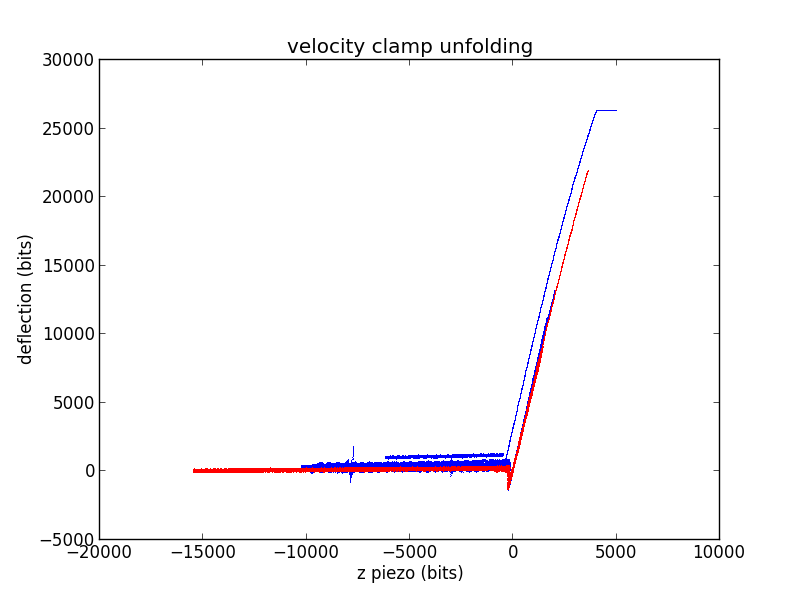
\includegraphics[width=0.9\textwidth]{%
        figures/labview-comparison/full}}
    \caption{\protect\subref{fig:pyafm:labview-comparison:many}Several
      velocity clamp pulls using both the LabVIEW/Windows stack (blue)
      and the Comedi/Linux stack (red).  The contact voltage and
      pulling distance were not synchronized between the two
      experiments, and the raw data has been shifted to locate the
      contact point at the origin.  One LabVIEW/Windows curve has a
      flat deflection in the high-contact region, where the laser was
      deflected beyond the photodiode's working range.  This is
      probably due to a high approach setpoint, followed by surface
      drift during the binding phase, but is not relevant to the
      stack comparison.\label{fig:pyafm:labview-comparison}}
  \end{center}
\end{figure}

\begin{figure}
  \ContinuedFloat
  \begin{center}
    \subfloat[][]{\label{fig:pyafm:labview-comparison:single:contact}
      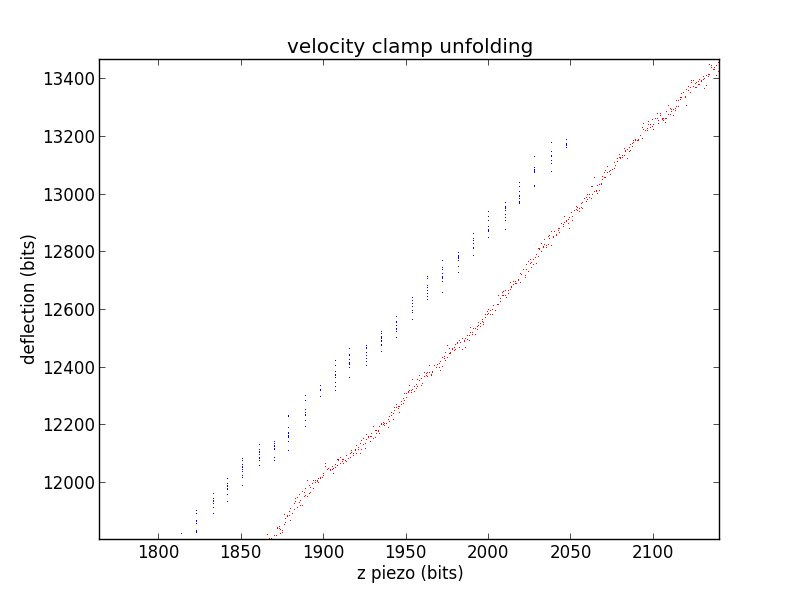
\includegraphics[width=0.9\textwidth]{%
        figures/labview-comparison/single-contact}} \\
    \caption{\protect\subref{fig:pyafm:labview-comparison:single:contact}The
      contact region from a single pull from
      \protect\subref{fig:pyafm:labview-comparison:many}.  The
      LabVIEW/Windows stack (blue) takes $0.5\U{nm}$ piezo steps with
      ten deflection reads at each step.  The Comedi/Linux stack (red)
      makes a single read per step, but can take as many small steps
      as possible within DAQ card's memory buffer, frequency, and
      precision limitations.  For $1\U{$\mu$m/s}$ pulls, a
      stepping/sampling frequency of $50\U{kHz}$ generated steps that
      were less than one DAC bit wide.}
  \end{center}
\end{figure}

\begin{figure}
  \ContinuedFloat
  \begin{center}
    \subfloat[][]{\label{fig:pyafm:labview-comparison:single:non-contact}
      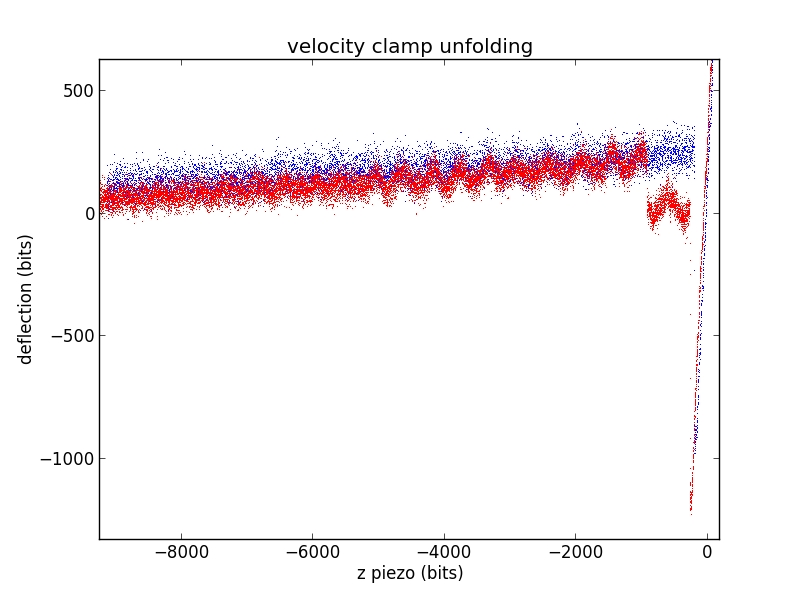
\includegraphics[width=0.9\textwidth]{%
        figures/labview-comparison/single-non-contact}}
    \caption{\protect\subref{fig:pyafm:labview-comparison:single:non-contact}The
      non-contact region from a single pull from
      \protect\subref{fig:pyafm:labview-comparison:many} using both
      the LabVIEW/Windows stack (blue) and the Comedi/Linux stack
      (red).  The signal oscillates because the AFM is sitting
      directly on the lab bench, our usual isolation mechanisms being
      unavailable when these curves were recorded.  All protein
      unfolding experiments were carried out with isolation, so the
      vibration was not a problem in those cases.}
  \end{center}
\end{figure}

Because the goal of these experiments was to compare the two software
stacks, the comparison was carried out using our standard AFM
cantilevers and gold surface, but distilled water was used instead of
PBS and no protein was bound to the surface.  This gives a simpler
system with fewer distracting features.  As shown in
\cref{fig:pyafm:labview-comparison,fig:pyafm:labview-comparison:stats},
large-scale features are identical, with similar contact slopes and
non-contact noise.

\begin{figure}
  \begin{center}
    \subfloat[][]{\label{fig:pyafm:labview-comparison:contact-slope}
      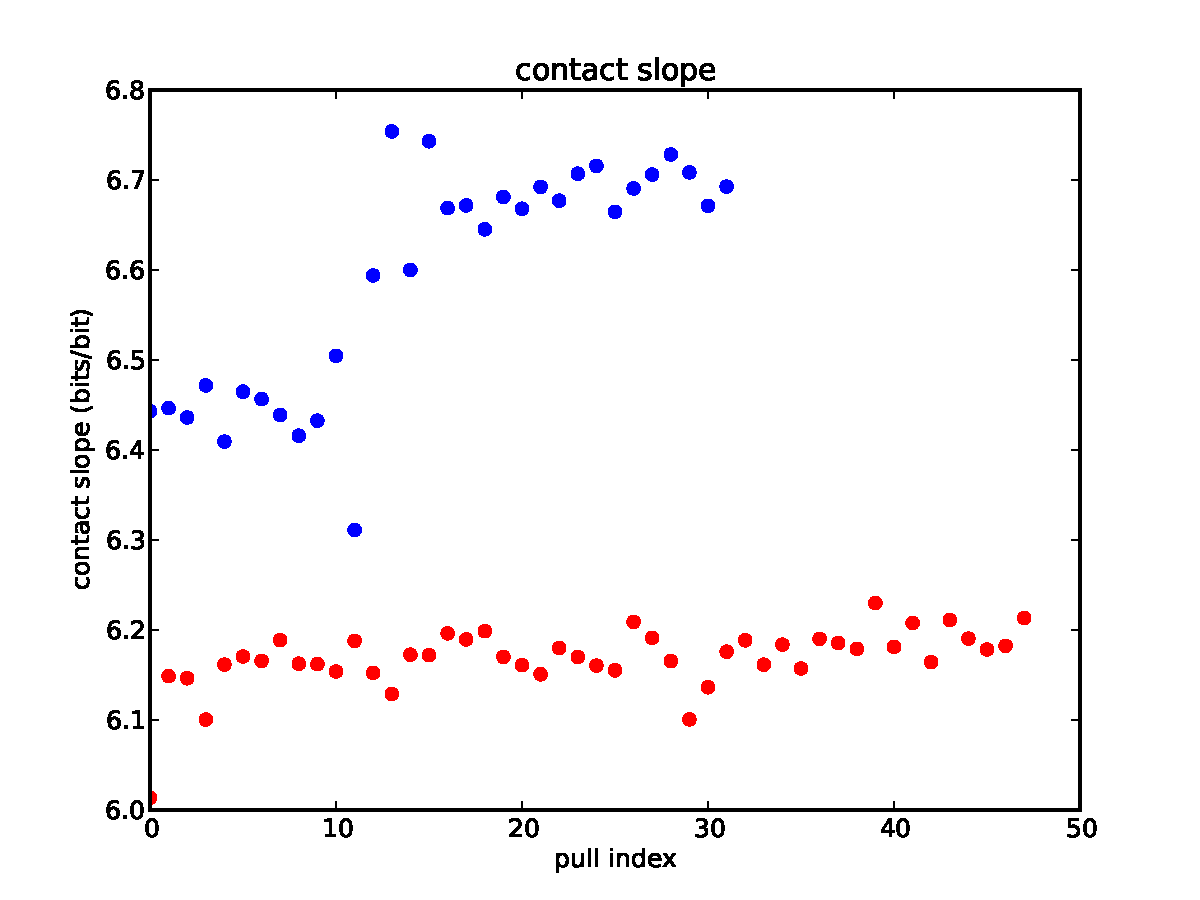
\includegraphics[width=0.5\textwidth]{%
        figures/labview-comparison/contact-slope}}
    \subfloat[][]{\label{fig:pyafm:labview-comparison:non-contact-noise}
      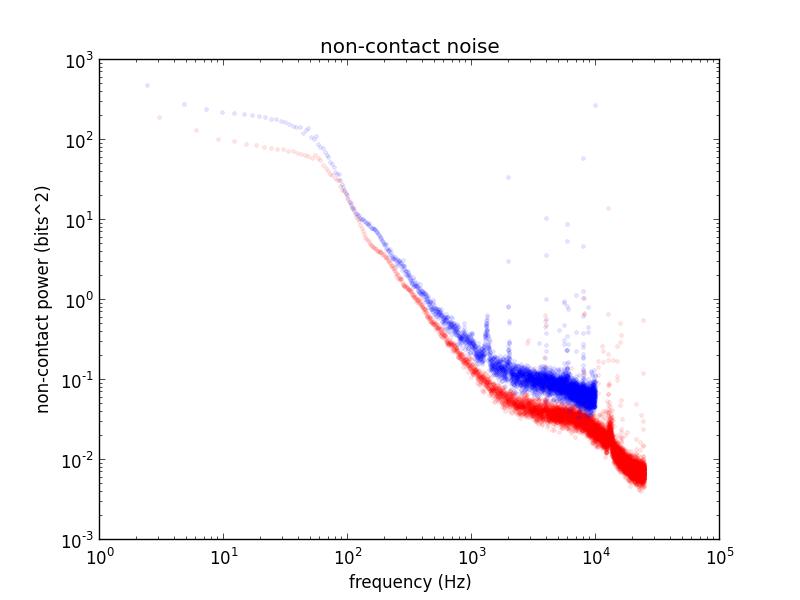
\includegraphics[width=0.9\textwidth]{%
        figures/labview-comparison/non-contact-noise}} \\
    \caption{\protect\subref{fig:pyafm:labview-comparison:contact-slope}Contact
      slope for the pull in \cref{fig:pyafm:labview-comparison} using
      both the LabVIEW/Windows stack (blue) and the Comedi/Linux stack
      (red).  The low-slope outlier is from the pull with out-of-range
      deflection.
      \protect\subref{fig:pyafm:labview-comparison:non-contact-noise}Power
      spectral densities (PSDs) of the non-contact noise for the pulls
      from \ref{fig:pyafm:labview-comparison:many}.  To produce this
      image, the PSD of the non-contact data extracted from
      \ref{fig:pyafm:labview-comparison:many} was averaged for each
      software stack.  The number of points in the non-contact region
      truncated to the nearest power of two (for efficient fast
      Fourier transformation), which has the convenient side effect of
      aligning the frequency axis for easy cross-pull
      averaging.\label{fig:pyafm:labview-comparison:stats}}
  \end{center}
\end{figure}

Although grossly similar, the two stacks do have some statistically
significant differences.  The slope of the contact region for the
LabVIEW/Windows stack (excluding the out-of-deflection-range outlier)
is $6.59\pm0.13$, while the Comedi/Linux stack slope is $6.17\pm0.03$
(both in deflection bits per $z$-piezo bit,
\cref{fig:pyafm:labview-comparison:contact-slope}).  While small, the
7\% difference is significant, both statistically ($3\sigma$ for the
LabVIEW/Windows standard deviation) and practically, because contact
slope plays a key role in cantilever calibration
(\cref{sec:calibcant:bump}).

Due to the table vibration, comparisons of non-contact noise between
the two stacks are less conclusive.  However, rough comparisons of the
noise spectra show that noise in the Comedi/Linux data is generally a
factor of two to three less than noise in the LabVIEW/Windows data
across a range of frequencies
(\cref{fig:pyafm:labview-comparison:non-contact-noise}).  While the
noise difference may be small, it does highlight the importance (and
difficulty) of characterizing your apparatus and controlling software.
